\documentclass[xcolor=dvipsnames, smaller]{beamer}

\usepackage[utf8]{inputenc}
\usepackage{amsmath, amsfonts}
\usepackage[francais]{babel}
\usepackage{hyperref, url, booktabs, subcaption, tikz}
%\usepackage{graphicx}
\hypersetup{colorlinks,linkcolor=black,urlcolor=violet}

\mode<presentation>{
  \setbeamertemplate{sections/subsections in toc}[square]
  \beamertemplatenavigationsymbolsempty
}

\newcommand{\N}{\mathbb{N}}                          % naturals
\newcommand{\set}[1]{\lbrace#1\rbrace}               % set
\newcommand{\R}{\mathbb{R}}         % real

\colorlet{darkred}{red!80!black}
\colorlet{darkblue}{blue!80!black}
\colorlet{darkgreen}{green!60!black}

\usetikzlibrary{calc,decorations.pathmorphing,patterns}
\pgfdeclaredecoration{penciline}{initial}{
    \state{initial}[width=+\pgfdecoratedinputsegmentremainingdistance,
    auto corner on length=1mm,]{
        \pgfpathcurveto%
        {% From
            \pgfqpoint{\pgfdecoratedinputsegmentremainingdistance}
                      {\pgfdecorationsegmentamplitude}
        }
        {%  Control 1
        \pgfmathrand
        \pgfpointadd{\pgfqpoint{\pgfdecoratedinputsegmentremainingdistance}{0pt}}
                    {\pgfqpoint{-\pgfdecorationsegmentaspect
                     \pgfdecoratedinputsegmentremainingdistance}%
                               {\pgfmathresult\pgfdecorationsegmentamplitude}
                    }
        }
        {%TO 
        \pgfpointadd{\pgfpointdecoratedinputsegmentlast}{\pgfpoint{1pt}{1pt}}
        }
    }
    \state{final}{}
}
%
\tikzstyle{block} = [draw,rectangle,thick,minimum height=2em,minimum width=2em]



% = = = = = = = = = = = = = = = = = = = = = = = = Separator = = = =

\AtBeginSection[]{
   \begin{frame}{Sommaire}
     \tableofcontents[currentsection]               
   \end{frame}
}

%--------------------------------------------------------------------------


\title{Non supervised classification of individual electricity curves} 
\author{Jairo Cugliari}
\institute{%Laboratoire ERIC, Université Lyon 2
%  \begin{center}
  %  
\includegraphics[height = 1.5cm]{pics/logo_dis.png}  
  %  ~~~~%  separator
  
\includegraphics[height = 1cm]{pics/logo_eric.png}  
%  ~~~~%  separator
%  
\includegraphics[height = 1cm]{pics/logo_lyon2.jpg} 
%\end{center}
}


\begin{document}

%--------------------------------------------------------------------------

% \begin{frame}[plain]

\begin{frame}[plain, noframenumbering, b]

% \begin{center}
% %  
\includegraphics[height = 1.5cm]{pics/logo_dis.png}  
% %  ~~~~%  separator
%   
\includegraphics[height = 1.5cm]{pics/logo_eric.png}  
%   ~~~~%  separator
%   
\includegraphics[height = 1.5cm]{pics/logo_lyon2.jpg} 
% \end{center}

\maketitle

  \begin{center}{\scriptsize 
    Joint work with Benjamin Auder (LMO, Université Paris-Sud) }
  \end{center}

  % \begin{flushright}
%    \includegraphics[width = 0.15\textwidth]{pics/by-nc-sa.png} 
% \end{flushright}
   
\end{frame}


% \maketitle
%   \begin{center}{\scriptsize 
%     Joint work with Benjamin Auder (LMO, Université Paris-Sud) }
%   \end{center}
% \end{frame}

%--------------------------------------------------------------------------

\frame{\frametitle{Outline}
       \tableofcontents
}

%--------------------------------------------------------------------------

\section{Motivation}


\begin{frame}{Industrial motivation}

\begin{columns}
\column{0.6\textwidth}
\begin{itemize}
 \item Smartgrid \& Smart meters : time real information
  \item Lot of data of different nature
 \item Many problems : transfer protocol, security, privacy, ...
 \item The French touch: 35M Linky smartmeter
\end{itemize}

\vskip 1cm

What can we do with all these data ?

\column{0.4\textwidth} 
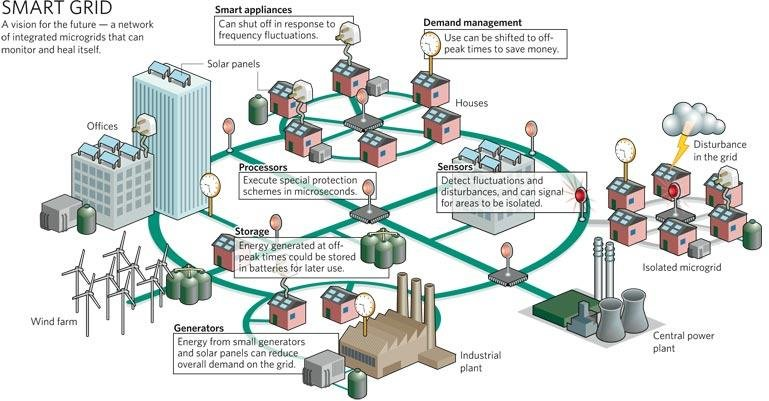
\includegraphics[width = \textwidth]{./pics/smartgrid.jpg} 

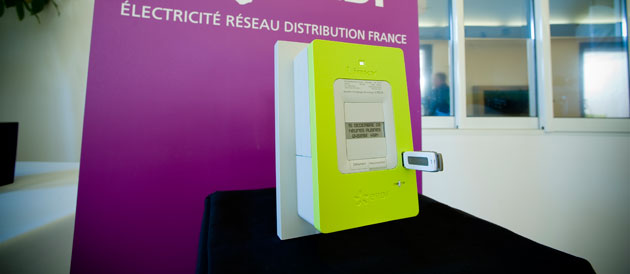
\includegraphics[width = \textwidth]{./pics/linky.jpg} 
\end{columns}
\end{frame}

%--------------------------------------------------------------------------

\begin{frame}{Electricity demand data}
\framesubtitle{Some salient features}

\begin{figure}[!ht] \centering
  \begin{subfigure}[t]{0.45\textwidth}
     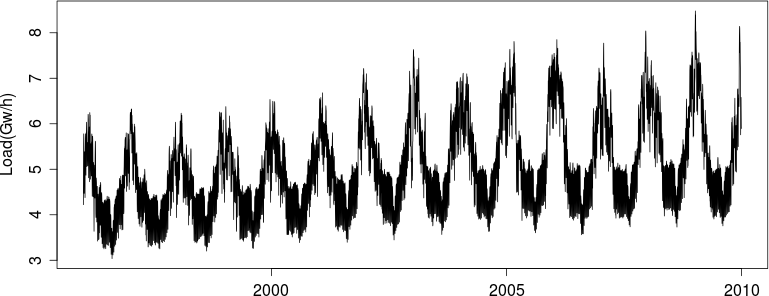
\includegraphics[width=\textwidth]{pics/longtermload.png}
     \caption{Long term trand} %\label{fig:gull}
  \end{subfigure}%
  ~ %spacing between images
  \begin{subfigure}[t]{0.45\textwidth}
     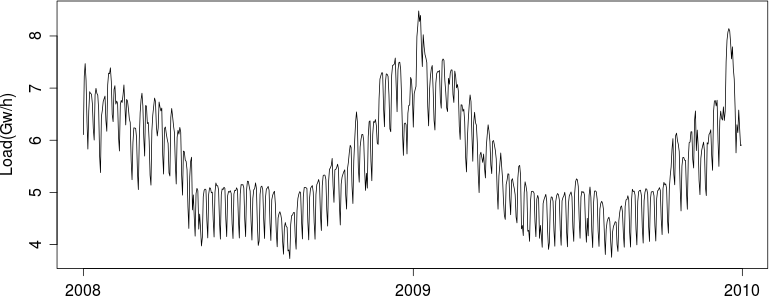
\includegraphics[width=\textwidth]{pics/twoyearsload.png}
     \caption{Weekly cycle} %     \label{fig:tiger}
  \end{subfigure}
  
  \begin{subfigure}[t]{0.45\textwidth}
     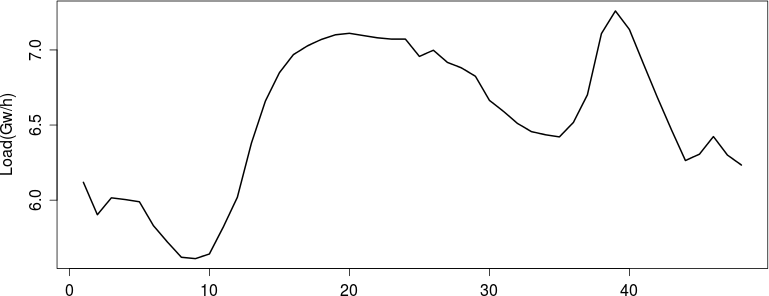
\includegraphics[width=\textwidth]{pics/dailyloads.png}
     \caption{Daily load curve} %   \label{fig:mouse}
  \end{subfigure}
  ~ %spacing between images
  \begin{subfigure}[t]{0.45\textwidth}
     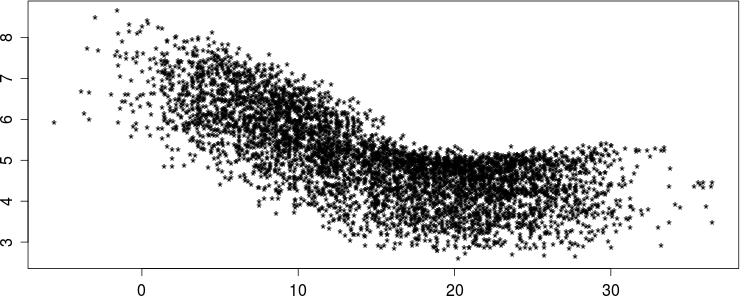
\includegraphics[width=\textwidth]{pics/consotemp.png}
     \caption{Electricity load vs. temperature}
  \end{subfigure}
\end{figure}
\end{frame}

%--------------------------------------------------------------------------

\begin{frame}[shrink]{FD as slices of a continuous process 
      \begin{scriptsize} \hfill [Bosq, (1990)] \end{scriptsize}} 
%  
  The prediction problem

\begin{itemize}
  \item Suppose one observes a square integrable continuous-time  stochastic process $X=(X(t), t\in\R)$ over the interval $[0,T]$, $T>0$;
  \item {We want to predict $X$ all over the segment $[T, T+\delta], \delta>0$}
  \item {Divide the interval into $n$ subintervals of equal
             size $\delta$.}
  \item Consider the functional-valued discrete time stochastic process $ Z = (Z_k, k\in\N) $, where $ \mathbb{N} = \set{ 1,2,\ldots } $, defined by 
\end{itemize}
 
\begin{columns}
  \column{5cm}    
      \begin{tikzpicture}[scale=0.5]
 
     % Axis
     \draw[<->, thick] (0,4) node (yaxis) [left] {$X_t$} 
        |- (11,0) node (xaxis) [right] {$t$} ;
     % Dashed grid
     \foreach \t in {1, 2, 3, 4, 5, 6} 
        \draw[dashed, color=PineGreen] (1.5*\t cm, 4) -- (1.5*\t cm, -3pt) 
                         node[anchor=north] {$\t \delta$};

     \draw[color=PineGreen] plot[smooth] file {tikz/data.dat};

     \draw (0,0) -- (0,-3pt) node[below, color= PineGreen] {0};
     \draw[dashed, color=PineGreen] (1.5*7,4) -- (1.5*7,-3pt) 
                         node[below] {};%$T+\delta$

     \foreach \t in {1, 2, 5} 
        \draw[color=PineGreen] (-0.75+1.5*\t, 1.5) node[below, scale=0.75] {$Z_\t(t)$};
        
     \foreach \t in {3, 4, 6} 
        \draw[color=PineGreen] (-0.75+1.5*\t, 3.5) node[below, scale=0.75] {$Z_\t(t)$};
     
  \end{tikzpicture} 

  \column{5cm} 
     \[ Z_k(t) = X(t + (k-1)\delta)             \]
     \[  k\in\N \;\;\; \forall t \in [0,\delta) \]
\end{columns}

\vfill
  If $X$ contents a $\delta-$seasonal component, 
     $Z$ is particularly fruitful.

\end{frame}

%--------------------------------------------------------------------------

\begin{frame}{Long term objective}

\begin{columns}
\column{.6\textwidth}
%\begin{figure}[!ht]\centering
  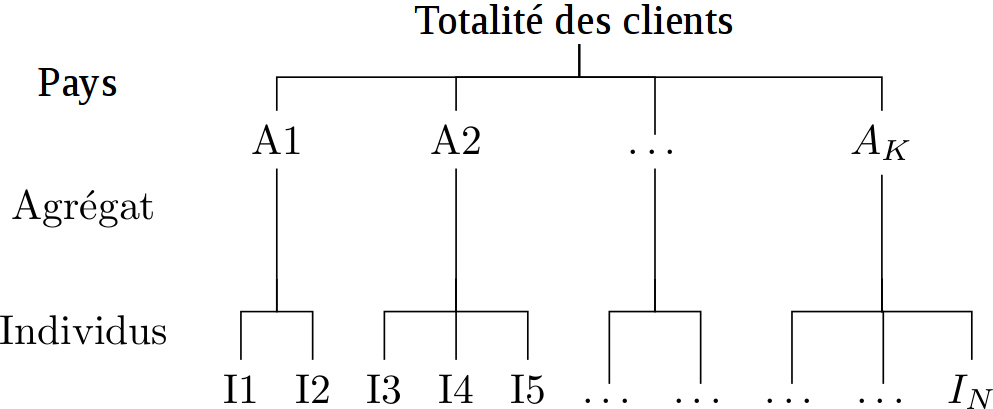
\includegraphics[width = \textwidth]{pics/schema.png} 
%\caption{Hierarchical structure of $N$ individual clients among $K$ groups.}\label{fig:schema-hier}
%\end{figure}
 
\column{.4\textwidth}
\begin{tikzpicture}[decoration=penciline, decorate]
  \node[block, decorate] at (0, 0){$Z_t$} ;
  \node[block, decorate] at (3, 0) {$Z_{t + 1}$} ;

  \node[block, decorate] at (0, -2.5) {$\begin{pmatrix}
                              Z_{t, 1} \\ Z_{t, 2} \\ \vdots \\ Z_{t, K}
                               \end{pmatrix}$ };

  \node[block, decorate] at (3, -2.5) {$\begin{pmatrix}
                           Z_{t+1, 1} \\ Z_{t+1, 2} \\ \vdots \\ Z_{t+1, k}
                               \end{pmatrix} $};

  \draw[decorate, darkblue,  line width = 2mm, ->] (1, 0) -- (2, 0);
  \draw[decorate, darkgreen, line width = 2mm, ->] (1, -2.5) -- (2, -2.5);
  \draw[decorate, black,     line width = 2mm, ->] (3, -1.3) -- (3, -0.4);
  \draw[decorate, darkred,   line width = 2mm, ->] (1, -1.5) -- (2, -0.75);
 \end{tikzpicture}
\end{columns}

\begin{itemize}
 \item Groups can express tariffs, geographical dispersion, client class ...
 \item \textbf{IDEA}: Use a clustering algorithm to learn groups of customer structure
 \item \textbf{Aim}: Set up a classical clustering algorithm to run in parallel 
\end{itemize}
\end{frame}

%--------------------------------------------------------------------------

\section{Functional clustering}

\begin{frame}{Aim}

\begin{columns}
  \column{0.6\textwidth}
  \begin{block}{ }
    \begin{itemize}
      \item Segmentation of $X$ may not suffices to render reasonable 
            the stationary hypothesis.
      \item If a grouping effect exists, we may considered stationary within each group. 
      \item Conditionally on the grouping, functional time series prediction methods 
            can be applied.
      \item We propose a clustering procedure that discover the groups from a bunch
             of curves.
    \end{itemize}

    We use wavelet transforms to take into account the fact 
    that curves may  present non stationary patters.
  \end{block}

  \column{0.4\textwidth}
    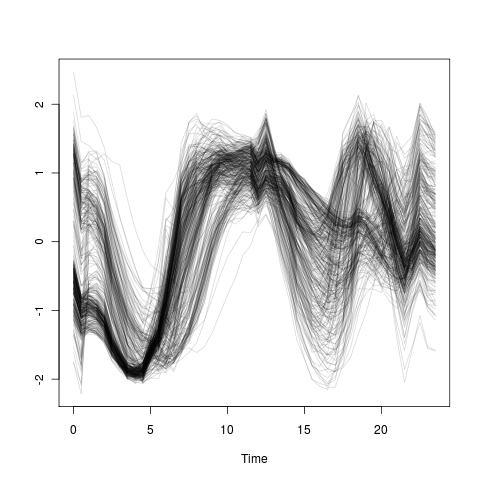
\includegraphics[width=0.9\textwidth,
                             height=2.7cm]{pics/conso-traj.png}

   Two strategies to cluster functional time series:
   \begin{enumerate}
     \item Feature extraction (summary measures of the curves).
     \item Direct similarity between curves.
   \end{enumerate}  

\end{columns}
\end{frame}

%---------------------------

\begin{frame}[plain]{Wavelets to cope with \textsc{fd}}

\begin{columns}
  \column{.6\textwidth}
 %\begin{figure}
 \centering
 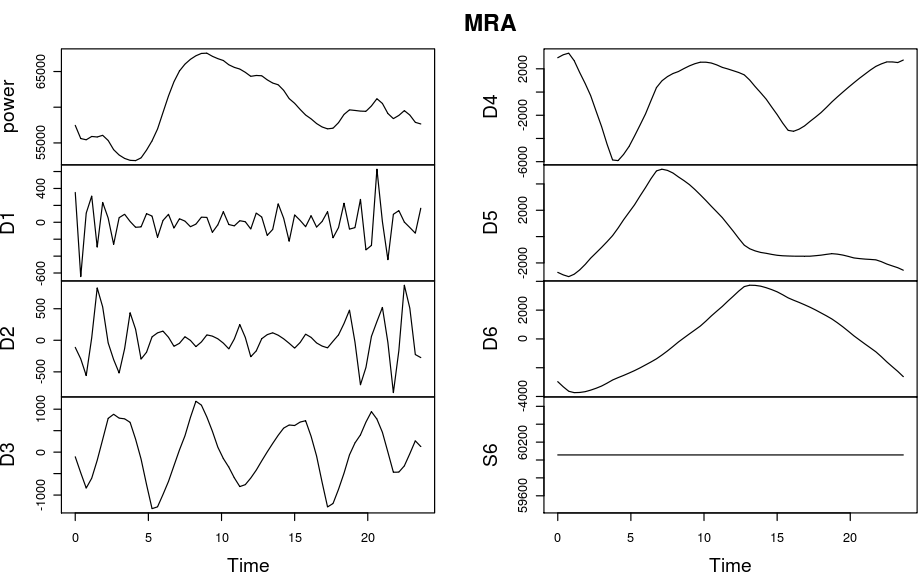
\includegraphics[width = \textwidth]{./pics/weekly-5.png}
  % * * * * * * * *  * * * * * * * * * * *
  \column{.4\textwidth}
\begin{block}{ } %Wavelet transform}
\begin{footnotesize}
\begin{itemize}
 \item domain-transform technique for hierarchical decomposing finite energy signals
 \item description in terms of a broad trend (\textcolor{PineGreen}{approximation part}), plus a set of localized changes kept in the \textcolor{red}{details parts}.
\end{itemize}
\end{footnotesize}
\end{block}
\end{columns}

\begin{block}{Discrete Wavelet Transform }

  If $z \in L_2([0, 1])$ we can write it as

   \begin{equation*}\label{eq:zeta}
     z(t) = \sum_{k=0}^{2^{j_0}-1} \textcolor{PineGreen}{c_{j_0, k}} \phi_{j_0,k} (t)  + 
        \sum_{j={j_0}}^{\infty} 
           \sum_{k=0}^{2^j-1} \textcolor{red}{d_{j,k}} \psi_{j,k} (t) ,
   \end{equation*}

%
where $ c_{j,k} = <g, \phi_{j,k} > $, $ d_{j,k} = <g, \varphi_{j,k}>$ are the 
\textcolor{PineGreen}{scale coefficients} and \textcolor{red}{wavelet coefficients} respectively, and the functions $\phi$ et $\varphi$ are associated to a orthogonal \textsc{mra} of $L_2([0, 1])$.
\end{block}
\end{frame}

%---------------------------------------- SLIDE ---------------------

\begin{frame}{Energy decomposition of the DWT}

\begin{block}{ }
 \begin{itemize}
  \item Energy conservation of the signal
%
  \begin{equation*}\label{eq:energy}  
     \| z \|_H^2    \approx     \| \widetilde{z_J} \|_2^2 
        = c_{0,0}^2 + \sum_{j=0}^{J-1} \sum_{k=0}^{2^j-1} d_{j,k} ^2  = 
                     c_{0,0}^2 + \sum_{j=0}^{J-1} \| \mathbf{d}_{j} \|_2^2.
  \end{equation*}
%  \item characterization by the set of channel variances estimated at the output of the corresponding filter bank
 \item For each $j=0,1,\ldots,J-1$, we compute the absolute and 
 relative contribution representations by
%      
   \[ \underbrace{\hbox{cont}_j = ||\mathbf{d_j}||^2}_{\fbox{AC}}  
      \qquad  \text{and}  \qquad
       \underbrace{\hbox{rel}_j  = 
     \frac{||\mathbf{d_j}||^2}
          {\sum_j ||\mathbf{d_j}||^2 }}_{\fbox{RC}} .\]
 \item They quantify the relative importance of the scales to the global dynamic.
% \item Only the wavelet coefficients $\set{d_{j,k}}$ are used.
 \item RC normalizes the energy of each signal to 1.
\end{itemize}
\end{block}
\end{frame}
% =======================================

\begin{frame} 
  \frametitle{Schema of procedure}
  \begin{center}
   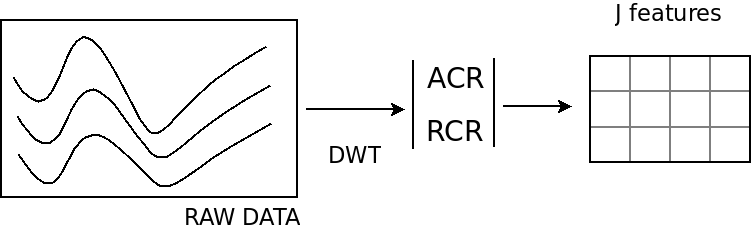
\includegraphics[width = 7cm, height = 2cm]{./pics/Diagramme1.png}
   % Diagramme1.png: 751x260 pixel, 72dpi, 26.49x9.17 cm, bb=0 0 751 260
  \end{center}
      
        \begin{footnotesize}
\begin{description}
 \item [0. Data preprocessing.] Approximate sample paths of $z_1(t),\ldots,z_n(t)$ %by the truncated wavelet series at the scale $J$ from sampled data $\mathbf{z}_1, \ldots, \mathbf{z}_n$.
 \item [1. Feature extraction.] Compute either of the energetic components using absolute contribution (AC) or relative contribution (RC).
 \item [2. Feature selection.] Screen irrelevant variables. \begin{tiny} [Steinley \& Brusco ('06)]\end{tiny}
 \item [3. Determine the number of clusters.] Detecting significant jumps in the transformed distortion curve.
 \begin{tiny} [Sugar \& James ('03)]\end{tiny}
 \item [4. Clustering.] Obtain the $K$ clusters using PAM algorithm.
\end{description}       \end{footnotesize}
    
\footnotetext[1]{Antoniadis, X. Brossat, J. Cugliari et J.-M. Poggi (2013), Clustering Functional Data Using Wavelets, {\it IJWMIP}, 11(1), 35--64}
    
\end{frame}

% ===========================================

\section{Parallel $k$-medoids}

\begin{frame}{Partitioning Around Medoids (PAM)
      \begin{scriptsize} \hfill [Kaufman et Rousseeuw~(1987)] \end{scriptsize}}

\begin{itemize}
 \item Partition the $n$ points $R^d$-scatter into $K$ clusters
 \item Optimization problem :
 \[ D(x) = \min_{m_1,\dots,m_k \in \mathbb{R}^d} \sum_{i=1}^{n} \min_{j=1,\dots,k} \| x_i - m_j \| \, ,\]
with $x = (x_1,\dots,x_n)$, $\|\,.\,\|$ can be any norm. Here we choose to use the euclidean norm. 
  \item Robust version of $k$-means
  \item Computational burden : medians instead of means
  \item Several heuristics allow to reduce the computation time.
\end{itemize}
\end{frame}

% ===========================================

\begin{frame}{Parallelization with MPI}

\begin{columns}
\column{.8\textwidth}
\begin{itemize}
 \item Easy to use library routines allowing to write algorithms in parallel
 \item Available on several languages 
 \item We use the master-slave mode
\end{itemize}

\column{.2\textwidth}

\includegraphics[width=\textwidth]{./pics/open-mpi-logo.png} 
\end{columns}

\vfill

\begin{block}{The outline of code:}
\begin{enumerate}
  \item The master process splits the problem in tasks over the data set and sends it to the workers;
  \item Each worker reduces the functional nature of the data using the DWT, applies the clustering and returns the centers;
  \item The master recuperates and clusters the centers into $K$ meta centers. 
\end{enumerate}
\end{block}

The source code is open and will be available to download from 
\href{https://github.com/}{github}.

\footnotetext[1]{B. Auder \& J. Cugliari. Parallélisation de l'algorithme des $k$-médoïdes. Application au clustering de courbes. (2014, submitted)}
\end{frame}

\section{Numerical experiences}

% ===========================================

\begin{frame}{Application I: Starlight curves}

\begin{itemize}
 \item Data from UCR Time Series Classification/Clustering
 \item 1000 curves learning set + 8236 validation set ($d= 1024$)% discretization points
\end{itemize}

\begin{figure}[H]
\begin{minipage}[c]{.32\linewidth}
	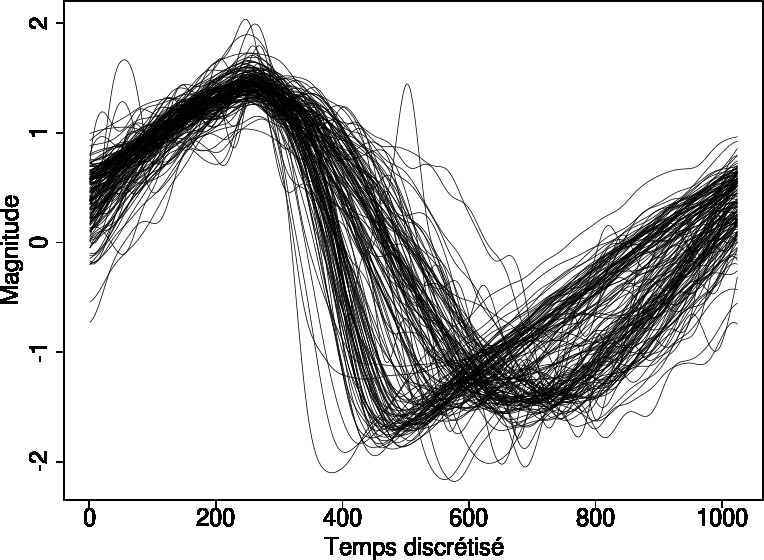
\includegraphics[width=\linewidth,height=3.5cm]{pics/slgr1.png}
	%\vspace*{-0.3cm}
	\caption{Groupe 1}
\end{minipage}
\begin{minipage}[c]{.32\linewidth}
	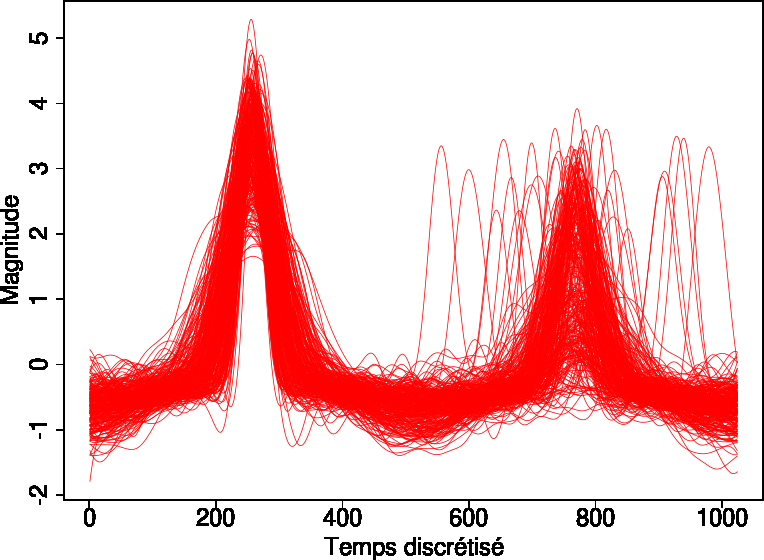
\includegraphics[width=\linewidth,height=3.5cm]{pics/slgr2.png}
	%\vspace*{-0.3cm}
	\caption{Groupe 2}
\end{minipage}
\begin{minipage}[c]{.32\linewidth}
	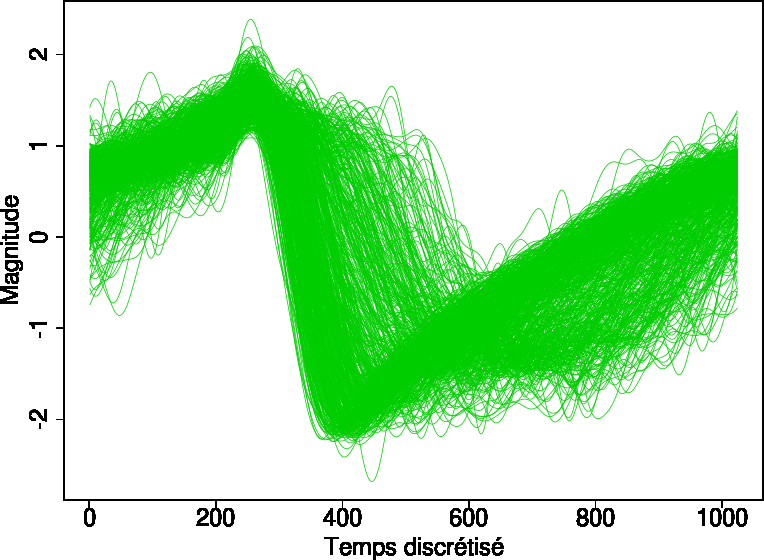
\includegraphics[width=\linewidth,height=3.5cm]{pics/slgr3.png}
	%\vspace*{-0.3cm}
	\caption{Groupe 3}
\end{minipage}
\label{figsltr3clusts}
\end{figure}

\begin{table}[H]
\centering
\begin{tabular}{lccc}                           \toprule
 &            & \multicolumn{2}{c}{Adequacy} \\
 & Distortion & Internal & External          \\ \midrule
Training (sequential) & 1.31e4 & 0.79 & 0.77 \\
Training (parallel)   & 1.40e4 & 0.79 & 0.68 \\
Test (sequential)     & 1.09e5 & 0.78 & 0.76 \\
Test (parallel)       & 1.15e5 & 0.78 & 0.69 \\ \bottomrule
\end{tabular}
%\caption{Distorsions et indices d'adéquation des partitions}
\label{tabDistorSl}
\end{table}
\end{frame}

% ++++++++++++++++++++++++++++++++++++++++++++++++++++++++++++++++

\begin{frame}{Application II: EDF data}
    \begin{figure}
    \centering
    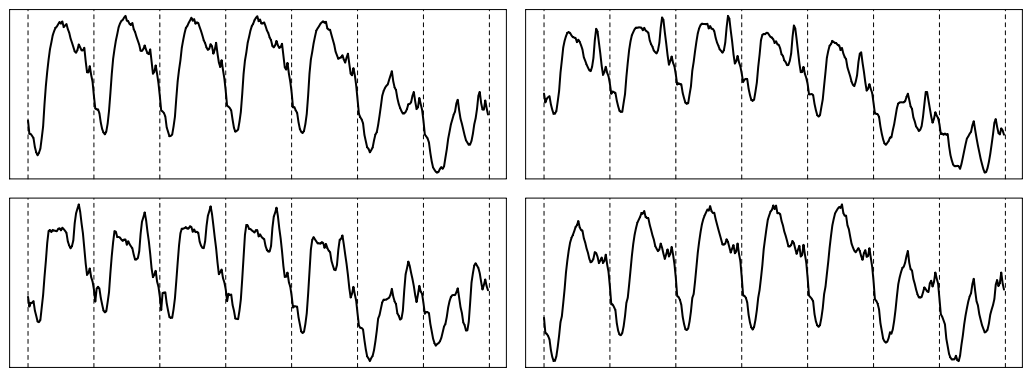
\includegraphics[width= 0.9\textwidth]{pics/conso-shapes.png}
    % conso-traj.eps: 0x0 pixel, 300dpi, 0.00x0.00 cm, bb=18 18 577 824
    \caption{  \begin{footnotesize}
French electricity power demand on autumn (top left), winter (bottom left), spring (top right) and summer (bottom right). \end{footnotesize} }
    \label{fig:conso-shapes}
    \end{figure}
    
    \begin{footnotesize}
 Feature extraction:
  \begin{itemize}
    \item The significant scales for revealing the cluster structure are independent of the possible number of clusters.
    \item Significant scales are associated to mid-frequencies. 
    \item The retained scales parametrize the represented cycles of 1.5, 3 and 6  hours (AC). 
 \end{itemize}                              \end{footnotesize}
\end{frame}


% ===========================================

\begin{frame}
\begin{figure}
  \centering
  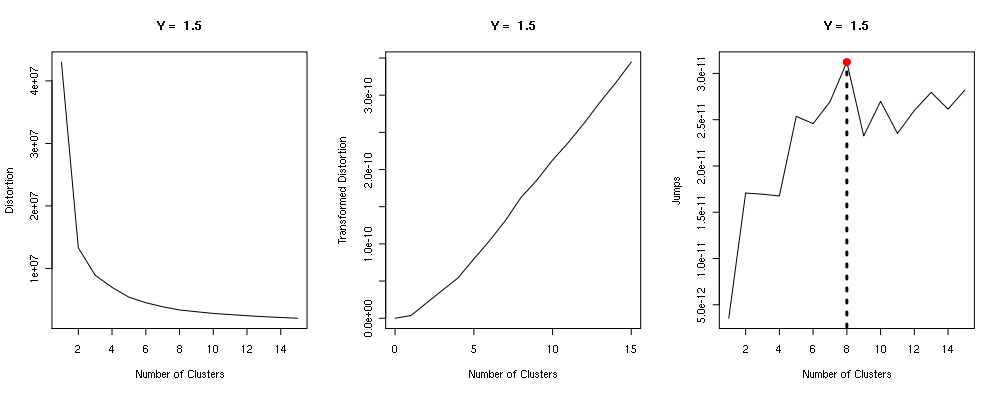
\includegraphics[width= 0.9\textwidth]{./pics/conso_jump_AC.png} \\
  \caption{ \begin{footnotesize}
Number of clusters by feature extraction of the AC (top). From left to right:  distortion curve, transformed distortion curve and first difference on the transformed distortion curve. \end{footnotesize} }
  \label{fig:conso-jumps}
\end{figure}
 \end{frame}

% ===========================================

\begin{frame}
\begin{figure} \centering
  \begin{subfigure}[t]{0.45\textwidth}
    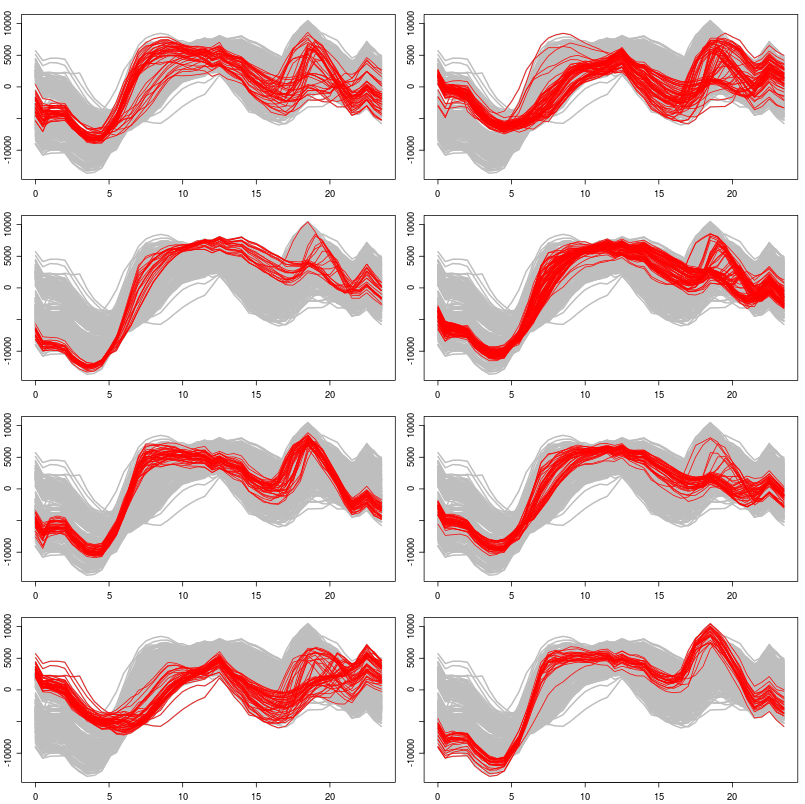
\includegraphics[width=\textwidth]{./pics/conso_AC-curves.png}
    \caption{Cluster}
  \end{subfigure}
  ~  	
  \begin{subfigure}[t]{0.45\textwidth}
    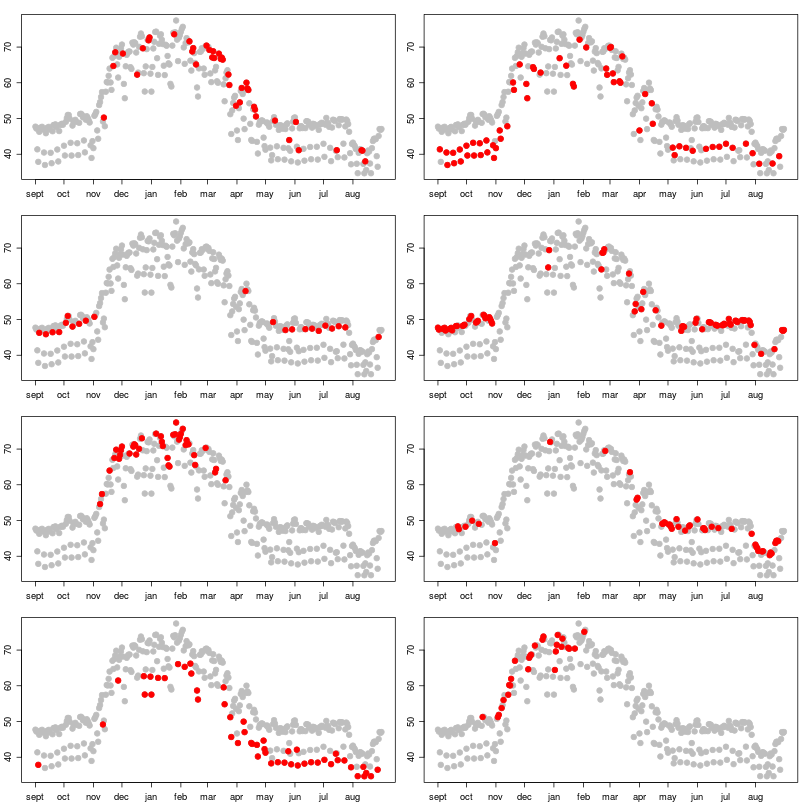
\includegraphics[width=\textwidth]{./pics/conso_AC-calendar.png}
    \caption{Calendar}
  \end{subfigure}
%      \subfloat[Calendar]{\label{fig:conso_clust_AC_cal}
%  	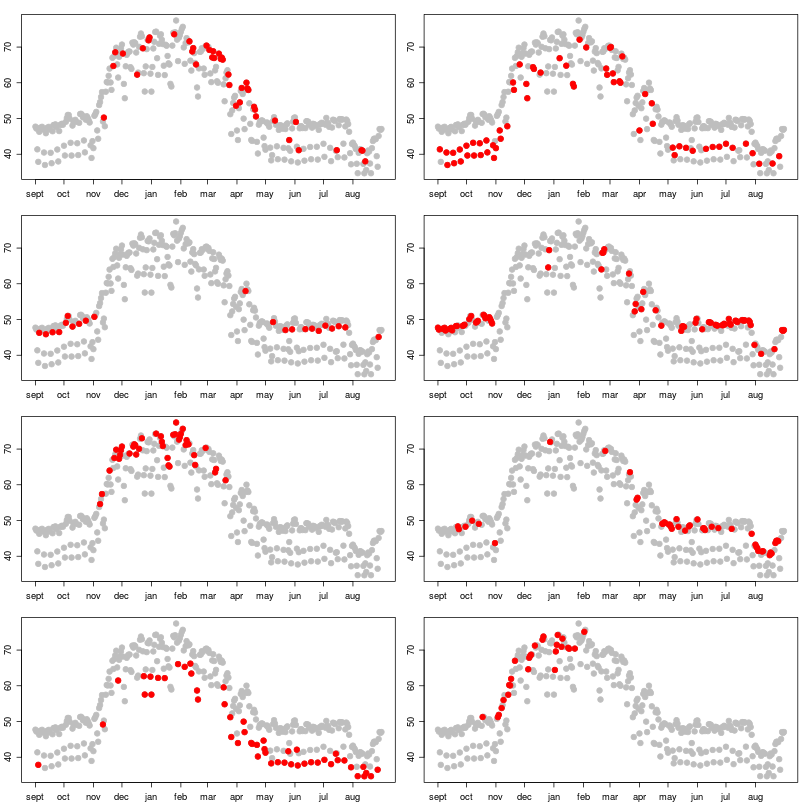
\includegraphics[width = 0.45\textwidth]{./pics/conso_AC-calendar.png}}                    
\caption{Curves membership of the clustering using AC based dissimilarity (a) and the corresponding calendar positioning (b).}
  \end{figure}
\end{frame}


% ===========================================


\begin{frame}{Application III: Electricity Smart Meter CBT (ISSDA)} \small

\footnotetext[1]{\textit{Irish Social Science Data Archive}, \url{http://www.ucd.ie/issda/data/}}

\begin{itemize}
 \item 4621 Irish households smart meter data % eséries de consommation électrique de foyers irlandais
 \item About 25K discretization points 
 \item We test with $K=$ 3 or 5 classes
 \item We compare sequential and parallel versions 
\end{itemize}


\begin{table}[H]
\centering
\begin{tabular}{lcc}                       \toprule
% &            &       \\
 & Distortion & Internal adequacy  \\ \midrule
3 clusters sequential & 1.90e7 & 0.90   \\
3 clusters parallel   & 2.15e7 & 0.90   \\
5 clusters sequential & 1.61e7 & 0.89   \\
5 clusters parallel   & 1.84e7 & 0.89   \\ \bottomrule
\end{tabular}
%  \caption{Distorsions et indices d'adéquation des partitions}
\label{tabDistorIr}
\end{table}

\end{frame}

%--------------------------------------------------------------------------

\section{Conclusion}

\begin{frame}{Conclusion}

\begin{itemize}
 \item Identification of customers groups from smartmeter data
 \item Wavelets allow to capture the functional nature of the data
 \item Clustering algorithm upscale envisaged for millions of curves
 \item \textit{Divide-and-Conquer} approach thanks to MPI library %pour l'algorithme des $k$-médoïdes : d'abord  sur des groupes de données courbes, puis des groupes de médoïdes jusqu'à obtenir un seul ensemble traité sur un processseur.
 %\item %Les résultats obtenus sur les deux jeux de données présentés sont assez encourageants, et permettent d'envisager une utilisation à plus grande échelle.
\end{itemize}

\begin{block}{Further work}
\begin{itemize}
 \item Go back to the prediction task
 \item Apply the algorithm over many hundreds of processors  
 \item Connect the clustering method with a prediction model
\end{itemize}
\end{block}
\end{frame}

%--------------------------------------------------------------------------

\begin{frame}[plain]{Bibliographie}\small

\begin{thebibliography}{10}
\bibitem{1} A. Antoniadis, X. Brossat, J. Cugliari et J.-M. Poggi (2013), Clustering Functional Data Using Wavelets, {\it IJWMIP}, 11(1), 35--64

\bibitem{2} R. Bekkerman, M. Bilenko et J. Langford - éditeurs (2011), Scaling up Machine Learning: Parallel and Distributed Approaches, {\it Cambridge University Press}

\bibitem{3} P. Berkhin (2006), A Survey of Clustering Data Mining Techniques, {\it Grouping Multidimensional Data, éditeurs : J. Kogan, C. Nicholas, M. Teboulle}.

\bibitem{6} J. Dean et S. Ghemawat (2004), MapReduce: Simplified Data Processing on Large Clusters, {\it Sixth Symposium on Operating System Design and Implementation}.

\bibitem{7} G. De Francisci Morales et A. Bifet (2013), G. De Francisci Morales SAMOA: A Platform for Mining Big Data Streams Keynote Talk at RAMSS ’13: 2nd International Workshop on Real-Time Analysis and Mining of Social Streams WWW, Rio De Janeiro

\bibitem{10} L. Kaufman et P.J. Rousseeuw (1987), Clustering by means of Medoids, {\it Statistical Data Analysis Based on the L\_1-Norm and Related Methods, éditeur : Y. Dodge}.
\end{thebibliography}
\end{frame}


\end{document}


% \begin{frame}{Motivation académique: Big Data} 
% \begin{itemize}
%  \item Besoins spécifiques: très grands volumes de données, grande dimension
%  \item Réponses: algorithmes opérant sur de grands graphes (Kang et al.~2009), sur des flux de données haut débit (De Francisci Morales et Bifet~2013)
%  \item Bekkerman et al.~(2011): algorithmes de Machine Learning s'exécutant en parallèle 
% \end{itemize}
% 
% \begin{itemize}
%  \item classification non supervisée (\textit{clustering}): regrouper les données en \textit{clusters} homogènes, suffisamment distincts deux à deux
%  \item nombreux algorithmes depuis Tyron~(1939) (voir Berkhin~2006 pour une revue) 
%  \item cependant la notion de cluster varie en fonction des données, du contexte et de l'algorithme utilisé
%  \item technique très populaire qui permet 
% de réduire la taille des données en les résumant à quelques représentants 
% \end{itemize}
% \end{frame}

